% !TeX root = ./main.tex

% TEMPLATE thesis UniPD

\documentclass[a4paper,12pt]{memoir} % memoir is book with abstract support


%%%%%%%%%%%%%%%%%%%%%%%%%%%%%%%%PACKAGES%%%%%%%%%%%%%%%%%%
\usepackage[font=small,labelfont=bf]{caption} %Makes image caption small
\usepackage[a-1b]{pdfx} % Generate a PDF/A

\pdfpagewidth\paperwidth
\pdfpageheight\paperheight

\usepackage[english]{babel} % [english]
\usepackage[utf8]{inputenc}
\usepackage[T1]{fontenc}

\usepackage{lmodern,amsmath,amssymb,graphicx}
%Subfloat figure
\usepackage{subfig}
\usepackage{wrapfig}
\usepackage{adjustbox}
\usepackage{graphicx} 

%inline code
\usepackage{listings}

\lstset{
	basicstyle=\ttfamily,
	columns=flexible,
}


%Wrapfigure
\usepackage{wrapfig}

%Tables
\usepackage{multirow}

% Useful for SI units:
\usepackage[per-mode=fraction,binary-units]{siunitx}

% Useful for bibliography:
\usepackage[style=alphabetic,natbib=false,doi=true,url=false, backend=bibtex]{biblatex}
\addbibresource{Bibliography/bibl}

% If you want to use subsections:
\setsecnumdepth{subsection}

\aliaspagestyle{chapter}{empty} % No page number on new chapter page

% Small margins:
\setulmarginsandblock{3cm}{*}{*}
\setlrmarginsandblock{2cm}{*}{*}
\checkandfixthelayout

\title{Inverse Beta Decay events selection in JUNO using Machine Learning algorithms}
\author{Candidate}
\date{Discussion date}

% METADATA for PDF
\begin{filecontents*}{\jobname.xmpdata}
\Title{Thesis title}
\Author{Candidate}
\Language{en-US} %{en-US}
\Date{YYYY-MM-DD}
\Keywords{keyword1\sep keyqord2\sep keyword3}
\end{filecontents*}

\hypersetup{hidelinks} % Hide link color boxes on pdf


\begin{document}

%%%%%%%%%%%%%%%%%%%%%%%%%%%%%%%%%%%%%% COVER %%%%%%%%%%%%%%%%%%%%%%%%%%%%%%%%%%%%%%
  \frontmatter
  \begin{titlingpage} % titlepage in book
    \vspace{5mm}
    \begin{figure}[ht]
      \centering
      
\includegraphics[scale=.13]{Images/logo.png}
    \end{figure}
    \vspace{5mm}
    \begin{center}
      {{\Large{\textsc{\textbf{UNIVERSITÀ DEGLI STUDI DI PADOVA}}}}\\}
      \vspace{5mm}
      {\textbf{Dipartimento di Fisica e Astronomia}} \\ % Department of XXXXXXXXXXXX
      \vspace{5mm}
      {\textsc{\textbf{Corso di Laurea Triennale in Fisica}}}\\ % Master's Degree in
      \vspace{20mm}
      {\textsc{\textbf{Tesi di Laurea}}}\\ % Final Dissertation
      \vspace{25mm}
      \begin{Spacing}{3}
        {\Large \textbf{\thetitle}}\\
      \end{Spacing}
      \vspace{8mm}
    \end{center}

    \vspace{15mm}
    \begin{Spacing}{1.5}
      \begin{tabular}{p{0.3\textwidth} p{0.3\textwidth} p{0.3\textwidth}}
        Relatore && Laureando\\ % Supervisor && Candidate
        \textbf{prof. Alberto Garfagnini} && \textbf{\theauthor}\\
        Correlatori && \textbf{Badge Number}\\ % Co-supervisors
        \textbf{dott. XXXXXX} && \\ % Dr.
        \textbf{dott. XXXXXX} && \\ % Dr.
      \end{tabular}
    \end{Spacing}
    \vspace{8 mm}
    \begin{center}
      \textbf{Anno Accademico YYYY/YYYY} % Academic Year
          \vspace{5 mm}\\\textbf{\thedate}
    \end{center}
  \end{titlingpage}
  \clearpage{\pagestyle{empty}\cleardoublepage}

%%%%%%%%%%%%%%%%%%%%%%%%%%%%%%%%%%%%%% ABSTRACT %%%%%%%%%%%%%%%%%%%%%%%%%%%%%%%%%%%%%%
  \begin{abstract}
   The Jiangmen Underground Neutrino Observatory (JUNO) will be the largest liquid scintillator-based neutrino detectors in the World, for the next decade. Thanks to its large active mass (20 kt) and state of the art performances (3\% effective energy resolution at 1 MeV), it will be able to perform important measurements in neutrino physics. The proposed thesis will study the application of different Machine Learning inspired algorithms for the discrimination of signal events (interactions of anti-neutrinos coming from the nearby nuclear power plants) from background events.
  \end{abstract}
  \newpage
% If abstract is required also in another language:
% requires: \usepackage[italian, english]{babel}
%   \begin{otherlanguage}{italian}
%     \begin{abstract}
%       Abstract in second language.
%     \end{abstract}
%   \end{otherlanguage}
%   \newpage

%%%%%%%%%%%%%%%%%%%%%%%%%%%%%%%%%%%%%% TABLE OF CONTENTS %%%%%%%%%%%%%%%%%%%%%%%%%%%%%%%%%%%%%%

  \tableofcontents
  \newpage
  %\listoffigures
  %\listoftables

%%%%%%%%%%%%%%%%%%%%%%%%%%%%%%%%%%%%%% BODY %%%%%%%%%%%%%%%%%%%%%%%%%%%%%%%%%%%%%%

  \mainmatter

  \chapter{Introduction}
\section{Neutrinos Oscillation}
The Standard Model of elementary particle interactions provides an accurate description of strong, weak, and electromagnetic interactions, but it treats these interactions as distinct and unrelated. Within this framework, neutrinos are assumed to be massless, but this assumption has been called into question by physicists. Neutrino oscillations, which occur when neutrinos change from one flavor to another, are a potential indication of neutrino mass.\\
The term "neutrino oscillations" refers to this phenomena and it involve the conversion of a neutrino of a particular flavor to another as it propagates through space.

Each known flavor eigenstate, $(\nu_e,\nu_{\mu},\nu_{\tau})$, linked to three respective charged leptons $(e,\mu,\tau)$  via the charged current interactions can be considered a complex combination of neutrino mass eigenstates as follow:

\begin{equation*}
	\left(\begin{array}{l}
		v_e \\
		v_\mu \\
		v_\tau
	\end{array}\right)=U_{\mathrm{PMNS}}\left(\begin{array}{l}
		v_1 \\
		v_2 \\
		v_3
	\end{array}\right)
\end{equation*}
in wich $\nu_i$ are the three mass eigensates, that have 3 masses  $m_i$  $(i = 1,2,3)$, which are non-degenerate, with $m_i \neq m_j$ for $i \neq j$.\\

The matrix $U_{\mathrm{PMNS}}$, called Pontecorvo-Maki-Nakagawa-Sakata (PMNS) matrix, is composed of three rotation matrices, $R_{23}$, $R_{13}$, and $R_{12}$, each corresponding to a different mixing angle, $\theta_{23}$, $\theta_{13}$, and $\theta_{12}$, respectively and a parameter $\delta_{CP}$ called the Dirac CP-violating phase. For this case, the Majorana $C P$ phases are $eta i(i=1,2)$, which are only physically possible if neutrinos are Majorana-type particles and do not participate in neutrino oscillations. Therefore, $U$ can be expressed as:

\begin{equation*} 
	\begin{split}
			U_{\text {PMNS }}&=\\
		=&\left(\begin{array}{ccc}
			1 & 0 & 0 \\
			0 & c_{23} & s_{23} \\
			0 & -s_{23} & c_{23}
		\end{array}\right) \left(\begin{array}{ccc}
			c_{13} & 0 & s_{13} \mathrm{e}^{-\mathrm{i} \delta_{C P}} \\
			0 & 1 & 0 \\
			-s_{13} \mathrm{e}^{\mathrm{i} \delta_{C P}} & 0 & c_{13}
		\end{array}\right) 
		\left(\begin{array}{ccc}
			c_{12} & s_{12} & 0 \\
			-s_{12} & c_{12} & 0 \\
			0 & 0 & 1
		\end{array}\right)\left(\begin{array}{ccc}
			\mathrm{e}^{\mathrm{i} \eta_1} & 0 & 0 \\
			0 & \mathrm{e}^{\mathrm{i} \eta_2} & 0 \\
			0 & 0 & 1
		\end{array}\right)
	\end{split}
\end{equation*}

The theoretical framework for neutrino oscillations involves the calculation of the oscillation probability as a function of the distance traveled by the neutrino, the neutrino mixing matrix, and the difference in squared masses between the three neutrino mass states, $\Delta m_{ij}^2$. Specifically,two nuclear power reactors 53 $\unit{\kilo\meter}$ away from the detector, which mostly produce anti-electron neutrinos $\bar{\nu}_e$ with energy below 10 MeV, are the principal sources of neutrinos for the JUNO experiment. So, it is necessary for the JUNO experiment to calculate the survival probability $P\left(\bar{\nu}_e \rightarrow \bar{\nu}_e\right)$ of electron antineutrinos.

\begin{equation*}
	P\left(\bar{\nu}_e \rightarrow \bar{\nu}_e\right)=1-\sin ^2 2 \theta_{12} c_{13}^4 \sin ^2\left(\frac{\Delta m_{21}^2 L}{4 \mathcal{E}}\right)-\sin ^2 2 \theta_{13}\left[c_{12}^2 \sin ^2\left(\frac{\Delta m_{31}^2 L}{4 \mathcal{E}}\right)+s_{12}^2 \sin ^2\left(\frac{\Delta m_{32}^2 L}{4 \mathcal{E}}\right)\right]
\end{equation*}

where $s_{i j} \equiv \sin \theta_{i j}, c_{i j} \equiv \cos \theta_{i j}, \mathcal{E}$ is the neutrino energy, $L$ the travelled distance and $\Delta m_{i j}^2 \equiv m_i^2-m_j^2$. \\
Past experiments have already given estimates for  $\Delta m_{21}^2,\left|\Delta m_{31}^2\right|$ and the  3 mixing angles.


\begin{figure}[h]
	\centering
	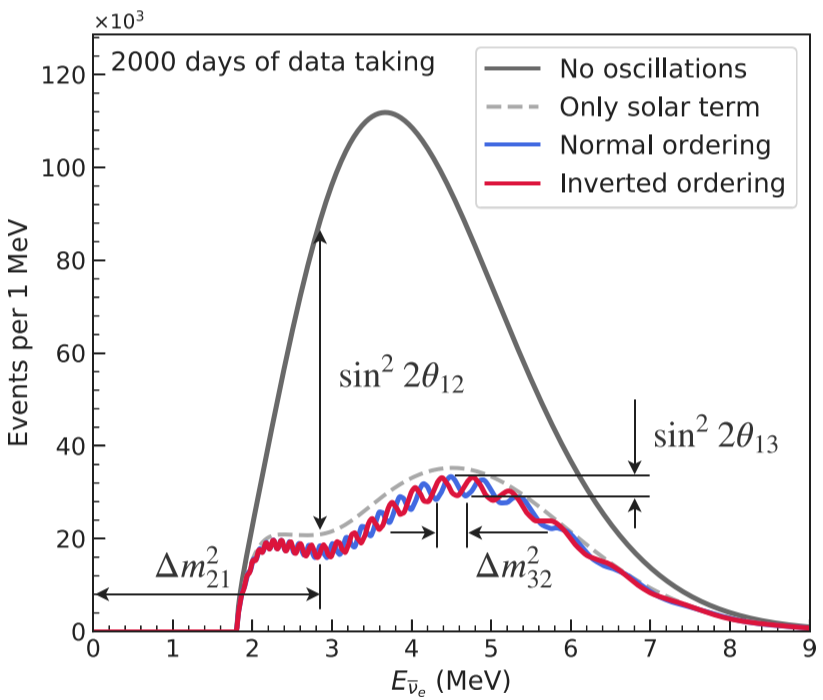
\includegraphics[width=0.4\linewidth]{Images/antineutino_to_antineutrino_probability_plot}
	\caption{JUNO's reactor antineutrino energy spectrum is shown with and without the effect of neutrino oscillation. The gray dashed curve includes only the term in the disappearance probability modulated by $sin^2(2\theta_{12})$, while the blue and red curves use the full oscillation probability for normal and inverted mass orderings. Spectral features driven by oscillation parameters are illustrated, highlighting the rich information available in JUNO's high-resolution measurement of the oscillated spectrum.}
	\label{fig:antineutinotoantineutrinoprobabilityplot}
\end{figure}


%TODO: Questo paragrafo da modificare come è scritto, FrMa
The aim of JUNO is then to improve these results, and especially fix the sign of $\Delta m_{31}^2$ by discriminating between two possibilities:\textit{ Normal Ordering} (\textbf{NO}), where $\left|\Delta m_{31}^2\right|=\left|\Delta m_{32}^2\right|+\left|\Delta m_{21}^2\right|$, and if $m_1<m_2<m_3$ we have the so called \textit{ Inverted Ordering} (\textbf{IO}), where $\left|\Delta m_{31}^2\right|=\left|\Delta m_{32}^2\right|-\left|\Delta m_{21}^2\right|$, and $m_3<m_1<m_2$.
In fact, depending on the sign of $\Delta m_{31}^2$, the plot of \ref{fig:antineutinotoantineutrinoprobabilityplot} is minimally different.


\section{The JUNO detector}

The Jiangmen Underground Neutrino Observatory (JUNO) is an experiment that is currently under construction in Southern China, in Jinji town, 43 km to the southwest of Kaiping city. This multipurpose experiment is expected to detect a large number of antineutrinos from nuclear reactors, with most of them originating from the Taishan and Yangjiang nuclear power plants (NPPs). These two plants are located at a baseline of about 52.5 km from the JUNO detector, which was optimized for the best sensitivity to the neutrino mass ordering, and have a combined nominal thermal power of 26.6 $GW_{th}$. JUNO requires knowledge of the unoscillated reactor antineutrino spectrum shape, which is why a specialized small detector named TAO will be situated approximately 30 meters from one of the Taishan reactors to precisely measure it. The data collected by TAO will serve as a data-driven input to restrict the spectra of the other reactor cores.\\


The JUNO detector comprises three main components, namely the Central Detector (CD), a water Cherenkov detector, and a Top Tracker (TT). The CD is a liquid scintillator (LS) detector, featuring an effective energy resolution of $\sigma_E/E =3\% / \sqrt{E (MeV)}$. It is composed of a 20 kton LS, enclosed within a spherical acrylic vessel, submerged in a water pool, that has a diameter of 43.5 m and a height of 44 m, providing sufficient buffer in all directions to protect the LS from the surrounding rock radioactivity. The water pool contains PMTs, which detect the Cherenkov light emitted from cosmic muons, acting as a veto detector.
The vessel is supported by a stainless steel (SS) structure, via Connecting Bars, with CD Photomultiplier Tubes (PMTs) installed on the inner surface of the SS structure. 
Compensation coils are mounted on the SS structure, aimed at suppressing the Earth's magnetic field and reducing its impact on the photoelectron collection efficiency of the PMTs. 
Atop the water pool lies a Top Tracker, which comprises a plastic scintillator array designed to precisely measure muon tracks. The CD is connected to the outside through a chimney, which facilitates calibration operations. The Calibration House, located above the chimney, contains special radioactivity shielding and a muon detector.\\

A schematic illustrating the location of both JUNO and TAO is shown in Fig. \ref{fig:junoschemeexperiment}.

\begin{figure}[h]
	\centering
	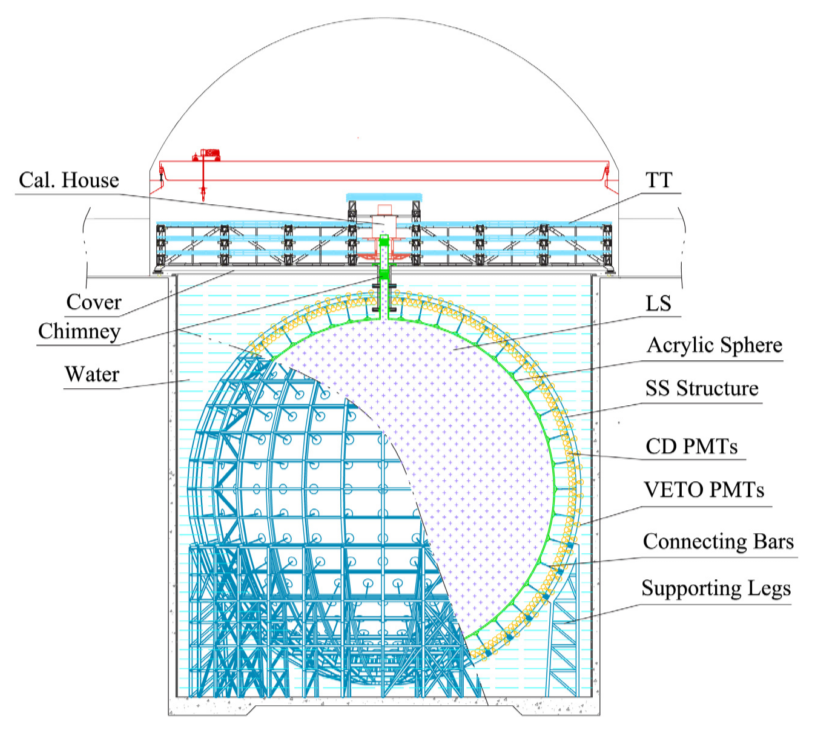
\includegraphics[width=0.7\linewidth]{Images/juno_scheme_experiment}
	\caption[JUNO scheme experiment]{Schematic view of the JUNO experiment}
	\label{fig:junoschemeexperiment}
\end{figure}


\section{JUNO signal and background}
\subsection{Signal}
%LIQUID SCINTILLATOR
The scintillator is doped with a small amount of gadolinium to enhance its sensitivity to antineutrinos via the inverse beta decay (IBD) process. The liquid scintillator used in JUNO is a combination of LAB (linear alkyl benzene) and PPO (2,5-diphenyloxazole) doped with a small amount of bis-MSB (1,4-bis(2-methylstyryl) benzene). When a neutrino interacts with the scintillator, it can produce charged particles such as electrons, protons, and alpha particles that travel through the scintillator and excite the scintillation molecules. This excitation results in the emission of photons with a wavelength of around 430 nm. These photons are detected by 20,000 20-inch photomultiplier tubes (PMTs) distributed in a 3-dimensional arrangement inside the detector.\\




\begin{equation}
	\begin{aligned}
		\overline{\nu}e + p &\rightarrow e^+ + n \\
		n + ^A_ZX &\rightarrow ^{A}_{Z-1}X^* + \gamma \\
		e^+ + e^- &\rightarrow 2\gamma
	\end{aligned}
\end{equation}

The PMTs detect the light and convert it into an electrical signal. The signals from all the PMTs are then combined to reconstruct the position and energy of the original neutrino interaction. This technique allows JUNO to measure the energy of the incoming neutrino to high precision, which is crucial for studying neutrino oscillation.

Moreover, the scintillator's composition and the detector's design are optimized to reduce background noise from other sources of radiation, such as cosmic rays and natural radioactivity. By carefully controlling these backgrounds, JUNO aims to achieve a signal-to-background ratio of better than 1:10,000, which is essential for observing the subtle effects of neutrino oscillation.

In JUNO's location, the energy spectrum will be distorted by two types of oscillations. The first is a slow (low frequency) oscillation driven by $\Delta m_{21}^2$ and modulated by $\sin ^2 \theta_{12}$, while the second is a fast (high frequency) oscillation driven by $\Delta m_{31}^2$ and modulated by $\sin ^2 \theta_{13}$. Fitting the data spectrum against the predicted spectrum distorted by standard neutrino oscillations enables measuring the oscillation parameters.\\
\subsection{Background}
Several different types of backgrounds signal are produced in the detector. For analysis we deeply analysed only the three most important contributes:


\paragraph{Radiogenic Backgrounds}

Radiogenic backgrounds arise from decays of radioactive isotopes in detector materials and surrounding rock. These decays can produce various forms of radiation, such as gamma rays and neutrons, which can interact with the detector and produce background events. Examples of radiogenic isotopes include $^{238}\mathrm{U}$, $^{232}\mathrm{Th}$, $^{40}\mathrm{K}$, and their daughter products. The main contributions to the radiogenic backgrounds come from the $^{238}\mathrm{U}$ and $^{232}\mathrm{Th}$ decay chains, with a smaller contribution from $^{40}\mathrm{K}$.

\paragraph{Cosmogenic Backgrounds}

Cosmogenic backgrounds arise from interactions of cosmic rays with materials surrounding the detector, such as the atmosphere and the Earth's crust. Muons produced in these interactions can penetrate the detector and produce background events. Specifically they interact with detector materials, producing isotopes such as $^{11}\mathrm{C}$, $^{9}\mathrm{Li}$, and $^{8}\mathrm{He}$, instable atoms which decay and produce additional background events.

\paragraph{Atmospheric Neutrino Backgrounds}

Atmospheric neutrino backgrounds arise from interactions of cosmic ray protons and nuclei with the Earth's atmosphere, which produce a flux of neutrinos that can interact with the detector. These interactions can produce both charged and neutral current events, which can mimic the signal from reactor neutrinos.

\paragraph{Reactor Antineutrino Backgrounds}

Reactor antineutrino backgrounds arise from the neutrinos produced in the nuclear reactors that power the JUNO experiment. These antineutrinos are the main signal for JUNO, but a small fraction of them can interact with the detector in ways that mimic background events. These interactions can produce both charged and neutral current events, which can be difficult to distinguish from the signal.


Here a viasualization sumary of all the bacgrounds contributions:

\begin{figure}[h]
	\centering
	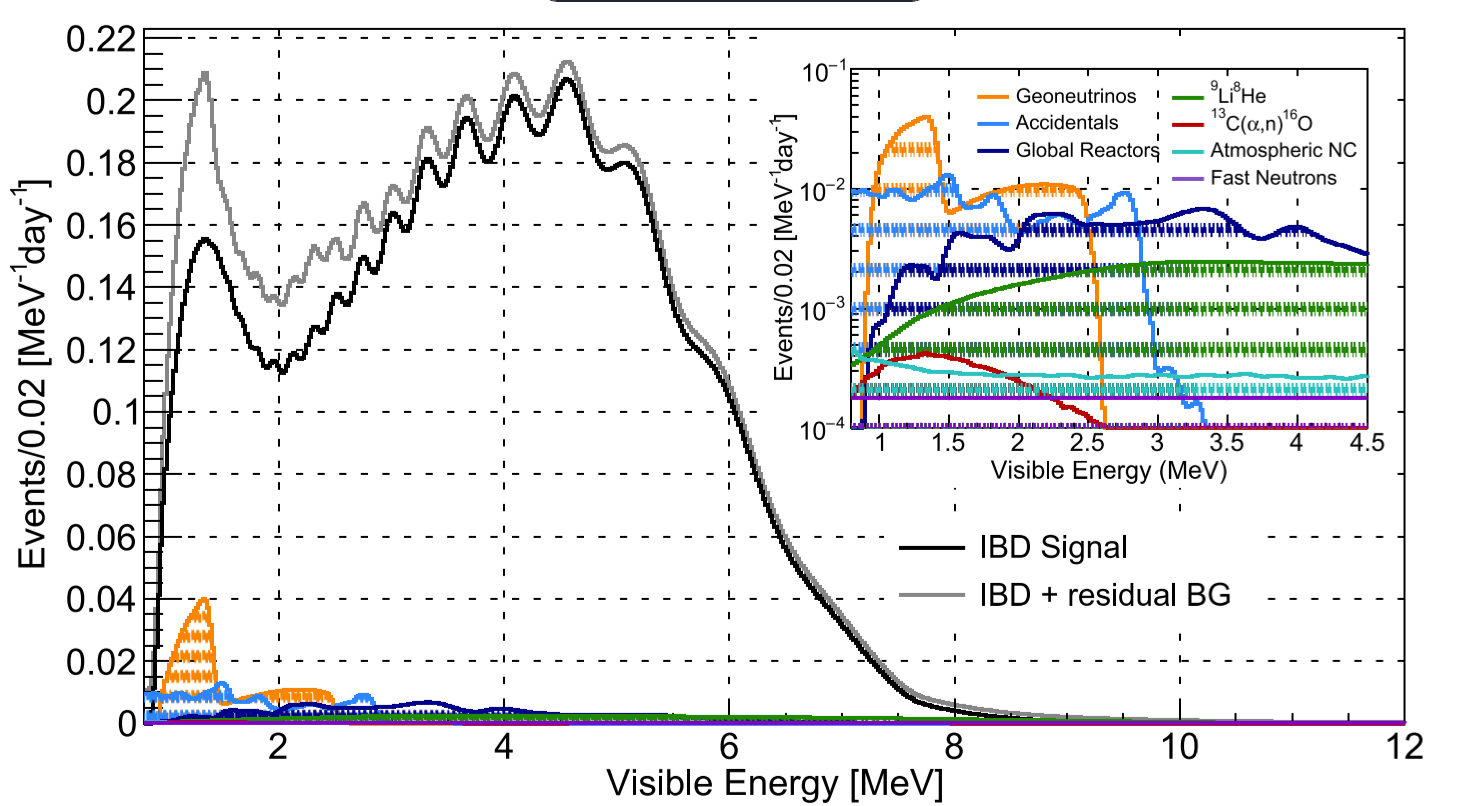
\includegraphics[width=0.7\linewidth]{Images/backgrounds_spectrum}
	\caption{Visible energy spectrum as measured by the LPMT system with (grey) and without (black) backgrounds is that which is anticipated for JUNO. The energy resolution is one of the assumptions listed in the text. The predicted backgrounds, which make up around 7$\%$ of the whole sample of IBD candidates and are primarily confined below, are shown in the inset as spectra. ~ 3 MeV}
	\label{fig:backgroundsspectrum}
\end{figure}

  \chapter{Frameworks}
\section{Introduction to Machine Learning}

Machine learning is a powerful tool that can be used to identify patterns in complex datasets. In the context of particle physics, machine learning algorithms can be used to detect signals from background noise in large datasets generated by detectors. In particular, for the detection of IBD signals from background, machine learning algorithms can be used to identify patterns in the data that are indicative of an IBD event, and to distinguish these signals from the background noise explained above.

\subsection{Supervised Learning}
Supervised learning, a cornerstone of machine learning, operates on the premise of training an algorithm using a labelled dataset. This training ensures that each input aligns with a correct output, with the overarching aim to develop a function that can link input data to output data accurately. A primary task stemming from supervised learning is binary classification, which is responsible for classifying elements of a dataset into one of two possible categories based on inherent features. In the context of this thesis, the emphasis is on applying the binary classification task to the JUNO experiment. The task is to distinguish whether a specific event is an Inverse Beta Decay (IBD) event or a background event.\\
 
Two distinct machine learning algorithms, \textbf{Gradient Boosting Decision Trees} and \textbf{Neural Networks}, are deployed to achieve this.

\section{Decision Tree}
A Decision Tree is a supervised machine learning algorithm used for classification and regression. It segments a dataset into subsets by applying decision rules inferred from the data's features. Each internal node represents a rule, dividing the data into two groups. The choice of rule is based on Information Gain, which relies on Entropy.

Entropy $H$ quantifies the impurity within a set $S$ and is defined as:

\begin{equation}
	H(S) = - p_{+} \log_{2}(p_{+}) - p_{-} \log_{2}(p_{-})
\end{equation}

Here, $p_+$ and $p_-$ denote the proportions of positive and negative instances in the set S, respectively. Entropy attains a maximum value when the set S contains an equal number of positive and negative instances, reflecting the highest uncertainty.

Information Gain (IG) measures the reduction in entropy achieved by partitioning the instances based on a feature (A). It is the difference between the entropy of the set before the split (H(S)) and the weighted sum of the entropies of each subset resulting from the split. It can be formulated as:

\begin{equation}
	IG(S, A) = H(S) - \sum_{v \in V(A)} \left(\frac{|S_v|}{|S|}\right) H(S_v)
\end{equation}

where $V(A)$ indicates the set of all possible values of feature A.\\
In this equation, $S_v$ denotes the subset of instances in S for which the feature A takes on the value v. $|S_v|$ and $|S|$ are the cardinalities of the sets $S_v$ and $S$, respectively.\\

The algorithm constructs the tree by recursively applying these splits, each time selecting the feature that results in the maximum information gain. This process continues until a stopping criterion is met, such as reaching a pre-specified maximum depth of the tree or a minimum number of samples per leaf.\\


While Decision Trees are straightforward and practical models, their ability to decipher complex patterns in data can be limited. This limitation paves the way for a more advanced technique known as Gradient Boosting Decision Trees. 

\subsection{Gradient Boosting Decision Trees}

 %[] https://www.youtube.com/watch?v=PxgVFp5a0E4&ab_channel=Prof.RyanAhmed
Gradient Boosting is a machine learning algorithm that stems from the concept of boosting, with the application of gradient descent methodology. Its goal is to produce a robust predictive model through the combination of multiple weak learners, typically decision trees.

The primary innovation in Gradient Boosting over classical boosting techniques is its approach to error correction. Instead of modifying the weights of misclassified instances, Gradient Boosting fits each new tree to the residuals (or the negative gradient) of the loss function with respect to the prediction of the existing ensemble of trees. This means each new tree is trained to predict the error of the existing model, thereby iteratively reducing the overall error.

Let's formalize this process:

\begin{enumerate}
	\item \textbf{Initialization}: We begin by initializing our model with a constant value. This is denoted as $F_0(x) = \arg\min_{\gamma} \sum_{i=1}^{N} L(y_i, \gamma)$, where $L(y, F(x))$ represents the loss function, $y$ represents the true target value, and $F(x)$ is the model's prediction for the input features $x$. This constant prediction, $\gamma$, is chosen to minimize the total loss over all $N$ instances. Thus, our initial model starts with a prediction that globally minimizes the loss.
	\item \textbf{Computation of Residuals}: Next, we iteratively construct an ensemble of $M$ trees. For each iteration $m=1$ to $M$, we calculate the residuals as
	\begin{equation}
		r_{im} = - \left[\frac{\partial L(y_i, F(x_i))}{\partial F(x_i)}\right]_{F(x)=F_{m-1}(x)}
	\end{equation} 
 	for each instance $i=1,2,...,N$. These residuals are essentially the negative gradients (or first derivatives) of the loss function with respect to the model's predictions. They provide a measure of the direction that would decrease the loss function fastest.
	\item \textbf{Fitting a Decision Tree}: After computing the residuals, we fit a new decision tree, $h_m(x)$, to these residuals. This tree is thus trained to predict the negative gradient of the loss function, using train it using the training set 
	${(x_i, r_{im})}_{i=1}^n$. By doing so, it attempts to correct the errors made by the current ensemble model.
	\item \textbf{Model Update}: The model is then updated by applying the rule
	\begin{equation}
		F_m(x) = F_{m-1}(x) + \nu \cdot h_m(x)
	\end{equation}
 	Here, $\nu$ represents the learning rate, a parameter typically less than 1, which controls the contribution of each tree to the final prediction. This essentially adjusts the previous model's prediction in the direction that most decreases the loss.
	\item \textbf{Final Model}: The final model's prediction is given by $F_M(x) = F_0(x) + \sum_{m=1}^{M} \nu \cdot h_m(x)$. In the final ensemble model, each decision tree provides a small correction to the predictions of the previous trees, collaboratively reducing the loss function's value and improving the overall model's performance.
\end{enumerate}


An advanced and highly efficient implementation of this method is XGBoost, which introduces several improvements such as parallel processing.


\section{Neural Networks}
Neural Networks (NNs) are computational models that draw inspiration from the interconnected structure of the human brain. Each individual computational unit, often referred to as an "artificial neuron" or simply "neuron", is designed to mimic the fundamental working mechanism of a biological neuron.

Let's denote the inputs to an artificial neuron as $ x = [x_1, x_2, ..., x_n] $, a representation analogous to dendrites in a biological neuron. These inputs are linearly transformed by a set of weights, $ w = [w_1, w_2, ..., w_n] $, summed together, and a bias term, $ b $, is added to the result. This operation can be expressed mathematically as:

\[
z = \sum_{i=1}^{n} w_i x_i + b 
\]

The calculated value, $ z $, is then passed through an \textit{activation function}, $ f $, to generate the neuron's output, $ a = f(z) $.


The activation function introduces non-linearity into the model, which is crucial for the network's ability to learn complex patterns. Common choices for $ f $ include the sigmoid, hyperbolic tangent, and ReLU (Rectified Linear Unit) functions.\\

An Artificial Neural Network builds upon the concept of the artificial neuron to form an interconnected assembly of these neurons, structured in layers. An ANN typically comprises an input layer, one or more hidden layers, and an output layer. Each layer may contain one or more neurons, and the layers are fully connected, meaning every neuron in one layer connects with all neurons in the following layer.

The following is a graphical representation of an ANN and a single neuron:

%TODO: Migliorare la qualità dell imagine, eliminare la parte scritta

\begin{figure}[h!]
	\centering
	
	\subfloat[Graphic representation of ANN]{
		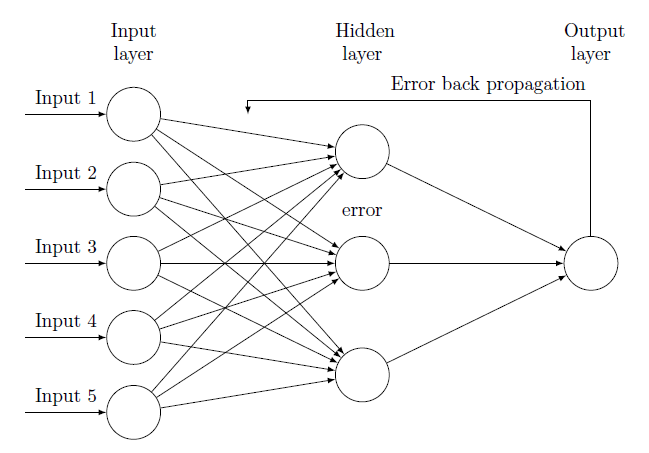
\includegraphics[width = 0.4\textwidth]{Images/fig_neural_network}
		\label{fig:nn_neuron}
	}
	\centering
	\subfloat[Single Neuron representation]{
		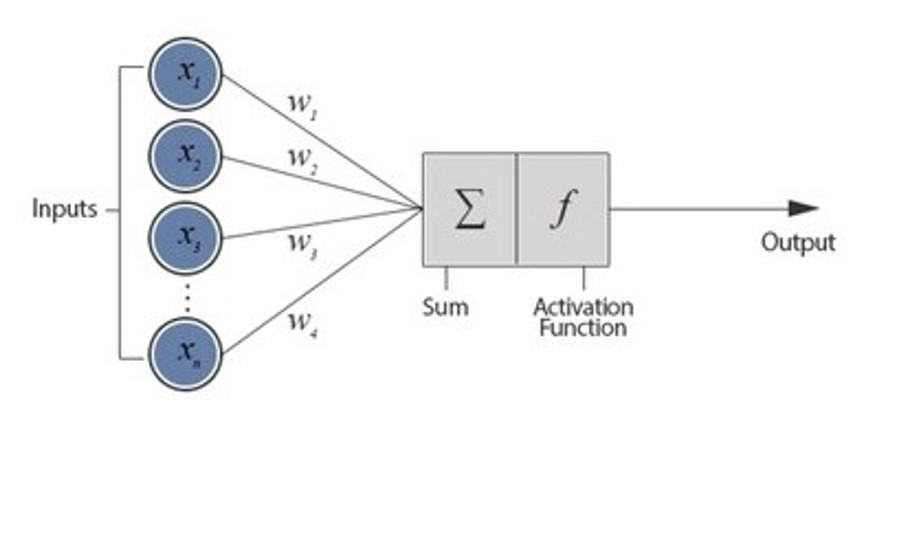
\includegraphics[width = 0.4\textwidth]{Images/nn_neuron}
		

	}
	
\end{figure}


For classification problems, the output layer typically uses a softmax function for multi-class problems to output a probability distribution over the classes, or a sigmoid function for binary classification problems to provide the probability of the positive class.

Training a neural network involves a two-step process: \textit{forward propagation} and \textit{backpropagation}. \\

In \textbf{forward propagation}, the input is passed through the network to generate an output. This output is then compared with the actual target to compute the loss function $ L $.

\textbf{Backpropagation} uses the chain rule of calculus to compute the gradient of $ L $ with respect to the network's parameters, which are then used to update the weights and biases:

\[
\frac{\partial L}{\partial w} = \frac{\partial L}{\partial a} \frac{\partial a}{\partial z} \frac{\partial z}{\partial w}
\]

Here, $ \frac{\partial L}{\partial a} $ is the derivative of the loss function with respect to the activation output, $ \frac{\partial a}{\partial z} $ is the derivative of the activation function, and $ \frac{\partial z}{\partial w} $ is the derivative of the weighted sum with respect to the weights.

Once these gradients are calculated, they are used to update the weights and biases via \textit{gradient descent}, a process that iteratively adjusts the parameters to minimize the loss function:

\[
w_{\text{new}} = w_{\text{old}} - \alpha \frac{\partial L}{\partial w}
\]

\[
b_{\text{new}} = b_{\text{old}} - \alpha \frac{\partial L}{\partial b}
\]

In these equations, $ \alpha $ is the learning rate, a hyperparameter that determines the size of the steps the algorithm takes down the gradient towards the minimum.

The interconnected structure of ANNs, combined with the ability of backpropagation and gradient descent to effectively adjust the model parameters, allows these networks to learn and represent complex, non-linear relationships in the data.

  \chapter{Analysis}

\section{Datasets}
The labeled datasets employed in the ensuing analysis are all products of Monte Carlo simulation, generated via the SNiPER software.

The first of the datasets provided is specifically tailored for the study of Inverse Beta Decay (IBD) events. Each event within this dataset, simulated and injected into the system, is tagged with a unique Simulation Identifier, or SimID. Furthermore, events which trigger a sufficient number of PMTs to be captured by the electronic system are assigned an EventID. This intricate labeling system allows for a clear differentiation between correlated IBD events, which represent actual IBD occurrences, and uncorrelated IBD events.


The second dataset focuses primarily on radioactivity events. Similar to the IBD dataset, it encompasses a large number of simulated events, each reflecting the complex reality of real-world physics phenomena. Additionally, the inherent electronic noise prevalent in actual physical environments is accurately accounted for, ensuring a realistic representation within the simulated context.

In this research undertaking, my central task will focus on a detailed examination and evaluation of the provided datasets. My work will primarily involve not just interpreting the inherent characteristics and peculiarities of the recorded events, but also harnessing these insights to construct comprehensive feature tables. These feature tables, generated from the datasets, will serve as the basis for my subsequent analysis and interpretation, a process which will be elaborated upon in the following sections of this study. The aim is to provide a meaningful understanding of the correlations and implications of these events within the broader context of the JUNO experiment.

%TODO-> Inserire il fatto che i dataset sono stati creati in ordine temporale in parallelo con SimID Per simulare 1500000 eventi nel MonteCarlo ci vorrebbero mesi e mesi di tempo macchina.
%Per affrontare il problema, si parallelizza la simulazione su una infrastruttura chiamata DCI (Distributed Computing Infrastructure).
%In questo modo si può ad esempio dividere i 1500000 eventi in 1500 jobs (simulati quindi da 1500 CPU diverse) da 1000 event ciascuno, completando la produzione in poche ore invece che in mesi.
%Questo approccio ha però il drawback che ogni simulazione parallela sarà indipendente dalle altre e quindi per ciascuna di queste il tempo, i SimID e tutte le altre quantità partirano da 0"" 

%La seconda colonna -> Si, sono il numero di eventi generati. Non tutti gli eventi generati interagiscono con il detector: un evento generato nella struttura metallica può venire fermato nella struttura stessa e non interagire con il detector, o ancora un evento generato nell'acrilico può venire emesso verso l'esterno e quindi non entrare mai in contatto con il detector e così via.
%Se consideri ora solo gli eventi che davvero sono entrati in contatto con il detector, non tutti gli eventi vengono ricostruiti: alcuni eventi sono così poco energetici che non sono sufficienti ad illuminare i PMT e quindi ad azionare il trigger per l'acquisizione dell'evento.

%Per darti un'idea, la rate di decadimenti radioattivi è circa 6.6 MHz, ne vengono effettivamente registrati dal detector appena 100 Hz (o poco meno)

%Questa è una delle sfide più grandi, perchè devi portare un segnale di circa 100 Hz (8.6 x 10e6 eventi/giorno) a rappresentare meno di 1 evento/giorno di background
%-------------------

%Nel MonteCarlo sono inclusi tutti gli effetti che ci aspettiamo nella realtà. E purtroppo, nella realtà, l'elettronica ha un rumore intrinseco (ad esempio puoi cercare in letteratura il Dark Count Rate per i PMTs).
%Ora, nel MonteCarlo vengono iniettati degli eventi (ad esempio una coppia prompt-delayed da IBD). A questo evento iniettato viene associato un SimID (simulation identifier) incrementale. Siccome prompt e delayed sono stati iniettati assieme, avranno lo stesso SimID.
%Non tutti gli eventi però sono registrati e salvati dall'elettronica. In JUNO, un evento viene salvato solo se questo è in grado di illuminare nello stesso momento un gran numero di PMTs (corrispondenti a qualche centinaio di keV).
%Se questo avviene, viene generato un trigger, viene salvato l'evento e gli viene associato un EventID incrementale.
%Può succedere che, per puro caso, il rumore intrinseco dell'elettronica "accenda" nello stesso momento un gran numero di PMT. In questo caso, nessun evento vero di fisica ha generato questo trigger, ma l'elettronica acquisisce e salva comunque questo evento, perch`ha superato la soglia di trigger. Quello che succede in questo caso è che l'evento avrà un EventID, ma nessun SimID associato, perchè nessun evento è stato davvero iniettato nella simulazione.
%Al contrario, può succedere che tu inietti una certa particella a cui quindi viene associato un SimID), ma questa non riesce a illuminare abbastanza PMT, l'evento non viene salvato e quindi non gli viene associato nessun EventID e non viene salvato nel file finale.


%Prima coppia simulata si becca SimID di 0. Gli Event IDs associati saranno 0 e 1.
%Seconda coppia generata avrà SimID di 1. EventIDs in questo caso sarnno 2 e 3. Ecc ecc.
%Sono incrementali per convenzione.

%TODO-> Spiega cosa c'è nei datasets -- ['EventID', 'SimID', 'timestamp', 't_sec', 't_nanosec', 'recx', 'recy', 'recz', 'm_QEn', 'm_pe']
%TODO-> Mention unbalanced datasets problem


%Ciao Fabio, la radioattività con cui hai lavorato rappresenta tutto il contributo da decadimenti radioattivi (alfa, beta, gamma) interno ed esterno a detector, ma che hanno depositato energia all'interno del detector.Ti lascio la tabella degli isotopi e delle rate di decadimento generate qui di seguito:

 

\begin{table}[htp]
\centering
\begin{tabular}{|c|c|c|}
	\hline
 \textbf{Dataset Name}  & \textbf{Number of Events}  & \textbf{Rates (used in elecsim)}   \\\hline\hline
      U238@LS      &   1,000,000 events    &           3.234 Hz            \\\hline
     Th232@LS      &   1,000,000 events    &           0.733 Hz            \\\hline
      K40@LS       &   1,000,000 events    &           0.53 Hz             \\\hline
     Pb210@LS      &   1,000,000 events    &           17.04 Hz            \\\hline
      C14@LS       & 1,000,000,000 events  &           3.3e4 Hz            \\\hline
      Kr85@LS      &   1,000,000 events    &           1.163 Hz            \\\hline
   U238@Acrylic    &   10,000,000 events   &           98.41 Hz            \\\hline
   Th232@Acrylic   &   10,000,000 events   &           22.29 Hz            \\\hline
    K40@Acrylic    &   10,000,000 events   &          161.25 Hz            \\\hline
   U238@node/bar   &  100,000,000 events   &          2102.36 Hz           \\\hline
  Th232@node/bar   &  100,000,000 events   &          1428.57 Hz           \\\hline
   K40@node/bar    &  100,000,000 events   &           344.5 Hz            \\\hline
   Co60@node/bar   &  100,000,000 events   &           97.5 Hz             \\\hline
   U238@PMTGlass   & 1,000,000,000 events  &          4.90e6 Hz            \\\hline
  Th232@PMTGlass   & 1,000,000,000 events  &          8.64e5 Hz            \\\hline
   K40@PMTGlass    & 1,000,000,000 events  &          4.44e5 Hz            \\\hline
  Tl208@PMTGlass   & 1,000,000,000 events  &          1.39e5 Hz            \\\hline
    Co60@Truss     &           0           &             ? Hz              \\\hline
    Tl208@Truss    &           0           &             ? Hz              \\\hline
 Rn222@WaterRadon  &  100,000,000 events   &            90 Hz              \\\hline
\end{tabular}
\caption{Here Caption}
\label{tab:BKG_gen}
\end{table}

\newpage

\section{Feature creation}
The development of machine learning models for the detection of Inverse Beta Decay (IBD) events necessitates a systematic and efficient approach to feature engineering. This process begins with the loading of two separate datasets, one for IBDs and one for radioactivity background, each containing a multitude of potential IBD events. The primary objective is to construct a feature table that encapsulates the unique characteristics of these events, providing a robust foundation for subsequent model training.

\subsection{IBD dataset}
As we mentioned earlier, an IBD event is characterized by two distinct signals with different energies, positions, and times. The first, known as the prompt signal, is caused by the annihilation of a positron with an electron in the scintillator liquid. This interaction yields a signal with a characteristic energy. The second, the delayed signal, results from the capture of a neutron by the scintillator liquid. This signal occurs with a significant delay, at a different position, and with a different energy compared to the prompt signal.

To create the feature table, all possible pairs of events within the dataset were considered, without repetition. Each possible combination was ordered temporally, meaning the second event followed the first. This temporal ordering is crucial in feature determination. Given a pair $i-j$, and considering that neutron capture occurs temporally subsequent to electron-positron annihilation, the following features were constructed:


\begin{itemize}
	 
	\item \textbf{$R_{prompt}$}: This feature represents the distance of the prompt signal, calculated as the distance from the origin to the point $(x_i, y_i, z_i)$ in the detector space where the prompt signal occurred.	
	
	\item $R_{delayed}$: Similar to $R_{prompt}$, this feature represents the distance of the delayed signal, calculated as the distance from the origin to the point $(x_j, y_j, z_j)$ in the detector space where the delayed signal occurred.

	\item \textbf{$E_{prompt}$}: This feature represents the energy of the prompt signal. It captures the characteristic energy released during the annihilation of a positron with an electron in the scintillator liquid.

	\item \textbf{$E_{delayed}$}: This feature represents the energy of the delayed signal. It captures the energy released when a neutron is captured by the scintillator liquid. This capture can occur by hydrogen, resulting in a gamma ray with an energy of approximately 2.2 MeV, or by carbon, resulting in gamma rays with combined energies of about 4.95 MeV to 5.12 MeV.

	\item \textbf{$\Delta_{Time}$}: This feature represents the time difference between the two events. It captures the temporal delay between the occurrence of the prompt and delayed signals.

	\item \textbf{$\Delta_{Radius}$}: This feature represents the spatial distance between the two events. It captures the spatial separation between the points in the detector space where the prompt and delayed signals occurred.

\end{itemize}
These features encapsulate the temporal and spatial differences between the prompt and delayed signals, as well as their respective energies, providing a comprehensive representation of the unique characteristics of IBD events.


\subsubsection*{Event Labeling}

In the context of supervised learning, the process of labeling is crucial as it provides the ground truth against which the performance of the machine learning model is evaluated. In this scenario, each pair of events in the dataset is assigned a label that indicates whether it represents a true Inverse Beta Decay (IBD) event or a background signal (BKG).

The label is a binary value: a label of 1 signifies a true IBD event, while a label of 0 signifies a BKG event. The assignment of these labels is not arbitrary but is guided by a specific criterion based on the simulation identifier (SimID) associated with each event pair.

The SimID is a unique identifier assigned to each simulated event pair during the generation of the dataset. If a pair of events share the same SimID, it means they were generated as part of the same simulation and thus are considered to represent a true IBD event. In this case, they are assigned a label of 1.

Conversely, if a pair of events do not share the same SimID, it means they were generated as part of different simulations. These events are not correlated and thus are considered to represent BKG events. In this case, they are assigned a label of 0.

This labeling strategy based on the SimID ensures a systematic and consistent methodology for event classification. It provides a clear and objective criterion to distinguish between true IBD events and BKG events, which is essential for the training and evaluation of the machine learning model.


\subsubsection*{Efficient Feature Calculation}
Given the large size of the dataset and the computational complexity of feature calculation, a parallel computing approach was adopted to enhance efficiency. The feature calculation task was divided into multiple sub-tasks that could be executed simultaneously by different cores of a CPU. This parallelization significantly reduced the total computation time, particularly beneficial when working with large volumes of data.


To further optimize the computation, a method was implemented to only consider event pairs where the delayed event occurs within a time window of $5*\tau$ from the prompt event. This approach is based on the fact that the time delay between the prompt and delayed events in Inverse Beta Decay (IBD) typically follows an exponential distribution, a characteristic of radioactive decay processes. While this method significantly reduces the number of potential event pairs, it might exclude about $0.7\%$ of IBD events that occur outside this time window. 

While this percentage is relatively small, it's important to consider the potential impact on the analysis results.

\subsection{Radioactivity dataset}
For the radioactivity dataset, the feature calculation was performed in a manner analogous to the IBD dataset. The key difference is that event pairs from the radioactivity dataset are labeled as BKG events, hence assigned a label of 0.



\begin{figure}[h]
	\centering
	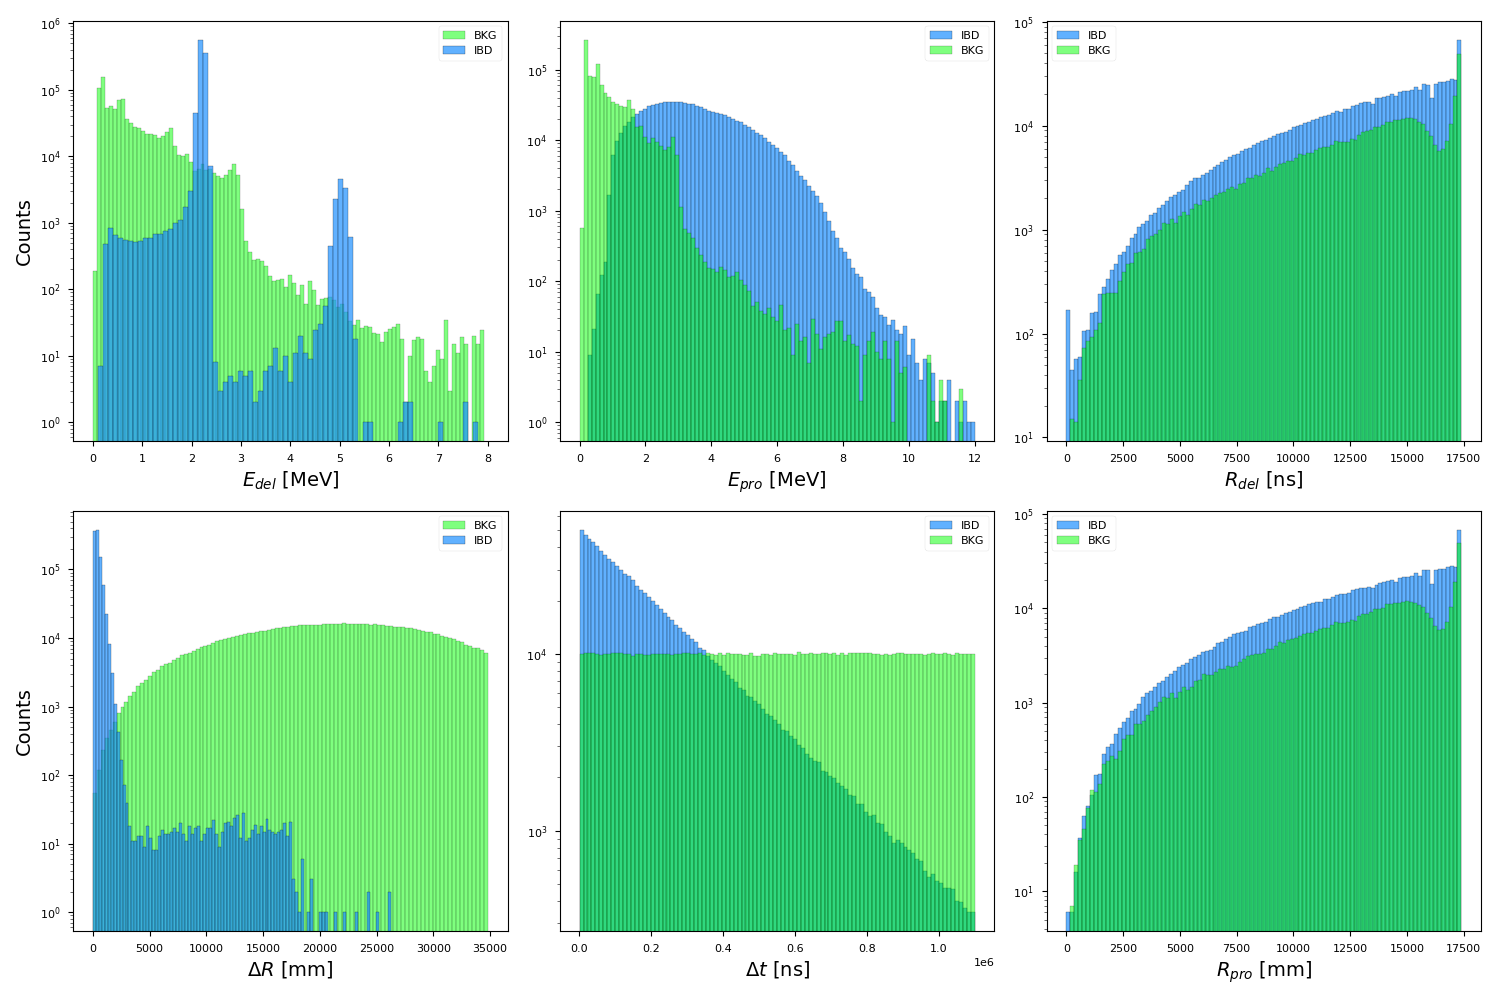
\includegraphics[width=1\linewidth]{Images/hist_features.png}
	\caption{Features histograms}
	\label{fig:hist_features}
\end{figure}



In summary, the feature engineering process for IBD event detection involves careful consideration of the unique characteristics of these events, systematic feature construction, and efficient computation strategies. This process provides a robust foundation for the development and training of machine learning models for IBD event detection.

\section{Models}


In the context of the JUNO experiment, a significant part of the effort involves the implementation and optimization of an event selection algorithm. The primary objective of this algorithm is to identify and select Inverse Beta Decay events induced by reactor antineutrinos, which are of paramount importance in the study of neutrino oscillations.

In this chapter, we will present several algorithms for event selection. The first algorithm is a manual cut-based approach, \textbf{Manual Cut}, where specific cuts are defined to select events of interest. This approach involves setting criteria based on the physical characteristics of the events and known background noise sources in the detector. The manual cut algorithm allows for precise control over the selection process and enhances the signal-to-background ratio.

In addition to the manual cut algorithm, other algorithms discussed in this chapter are based on machine learning models, specificaly based on \textbf{Boosted Decision Trees} and on \textbf{Neural Network}. 

The inclusion of machine learning algorithms in event selection provides an alternative approach that can adapt to complex and evolving data patterns. These algorithms can uncover subtle features in the data that may not be easily captured by manual cuts alone.

By exploring both manual cut and machine learning-based algorithms, we aim to provide a comprehensive understanding of different approaches to event selection, highlighting their strengths and limitations in the context of the JUNO experiment.

\subsection{Manual Cut}
The algorithm is designed to suppress various types of background noise while maintaining high efficiency for true IBD events. The selection criteria, or "cuts", are implemented using Python Code,and are applied to the Features Tables discussed above. Each cut within the algorithm serves a distinct purpose in the overall event selection process.

The key components of the event selection algorithm are as follows:

\begin{enumerate}
	\item \textbf{Delta Time ($\Delta t$) and Delta Radius ($\Delta R$) cuts}: The first cut is applied on the time delay and the radial distance between the prompt and delayed signals. The criteria are:
	\begin{itemize}
		\item Time separation between the prompt and delayed signals should be less than 1.0 ms.
		\item Spatial 3D separation should be less than 1.5 m.
	\end{itemize}

	These cuts are designed to reduce accidental background noise, which is the coincidence of two otherwise uncorrelated events, typically of radiogenic origin. The accidental background can be measured with excellent precision and subtracted by off-time window techniques. By imposing a limit on the time and spatial separation between the prompt and delayed signals, the algorithm can effectively distinguish between true IBD events and accidental coincidences.
	\item \textbf{Energy of the Prompt Signal ($E_{pro}$) Cut}: The next cut is applied on the energy of the prompt signal, which is the initial signal produced by the antineutrino interaction. The criteria are:
	\begin{itemize}
		\item Energy of the prompt signal should be within the [0.7, 12.0] MeV range.
	\end{itemize}
	
	This cut is based on the expectation that IBD events dominate this energy range. The energy of the prompt signal corresponds to the energy of the positron from the IBD reaction, and the specific range is chosen to maximize the signal-to-background ratio.
	\item \textbf{Energy of the Delayed Signal ($E_{del}$) Cut}: The final cut is applied on the energy of the delayed signal, which is the signal produced by the neutron capture that follows the antineutrino interaction. The criteria are:
	\begin{itemize}
		\item Energy of the delayed signal should be within the [1.9, 2.5] MeV or [4.4, 5.5] MeV ranges.
	\end{itemize}
	
	These energy selection windows correspond to neutron capture on hydrogen and carbon, respectively. The energy of the delayed signal is characteristic of the neutron capture process, and the specific ranges are chosen to correspond to the expected energies of neutron capture on hydrogen and carbon in the detector.
\end{enumerate}

An evaluation was conducted to assess the accuracy of the algorithm. In this evaluation, the feature table of true IBD events was utilized to gauge the algorithm's performance. The results indicated that out of a total of 1,468,385 events, 1,435,115 events were accurately classified as IBD. This achievement translates to an accuracy rate of $97.73\%$, indicating the algorithm's successful identification of the majority of true IBD events.\\


Furthermore, the efficiency calculation was performed on the background dataset, yielding the following results: 26.0 out of 993,457 events were mistakenly classified as IBD, resulting in an efficiency rate of $99.997\%$. This indicates that the algorithm has an excellent capability to distinguish and reject background events, achieving a high level of efficiency in identifying true IBD events. The extremely low misclassification rate of background events as IBD further highlights the algorithm's effectiveness in minimizing false positives and maintaining a high level of purity in the selected IBD events.


A summary table presents the results obtained from the evaluations:

\begin{table}[ht]
	\centering
	\caption{Summary of Algorithm Performance}
	\label{tab:algorithm-results}
	\begin{tabular}{|c|c|c|c|}
		\hline
		Dataset & Total Events & IBD Events Selected & Accuracy (\%) \\ \hline\hline
		True IBD Events & 1,468,385 & 1,435,115 & 97.73 \\ \hline
		Background Events & 993,457 & 26 & 99.997 \\ \hline
	\end{tabular}
\end{table}

\subsection{XGBoost}
\subsection{PyThorch}

\section{Conclusion}

% Please add the following required packages to your document preamble:
% \usepackage[table,xcdraw]{xcolor}
% If you use beamer only pass "xcolor=table" option, i.e. \documentclass[xcolor=table]{beamer}
\begin{table}[h!]
	\begin{tabular}{lllll}
		\cline{1-3}
		\multicolumn{1}{|l|}{} & \multicolumn{1}{c|}{{\color[HTML]{CE6301} \textbf{Manual Cut Algorithm}}} & \multicolumn{1}{l|}{{\color[HTML]{009901} \textbf{BDT Algorithm}}} &  &  \\ \cline{1-3}
		\multicolumn{1}{|l|}{\textit{Radioactivity}} & \multicolumn{1}{l|}{\begin{tabular}[c]{@{}l@{}}Efficiency: 99.9973\%\\ Purity: 100\%\end{tabular}} & \multicolumn{1}{l|}{\begin{tabular}[c]{@{}l@{}}Efficiency: 99.997684\%\\ Purity: 100\%\end{tabular}} &  &  \\ \cline{1-3}
		\multicolumn{1}{|l|}{\textit{True IBDs}} & \multicolumn{1}{l|}{\begin{tabular}[c]{@{}l@{}}Efficiency: 97.734\%\\ Purity:100\%\end{tabular}} & \multicolumn{1}{l|}{\begin{tabular}[c]{@{}l@{}}Efficiency: 99.997616\%\\ Purity: 100\%\end{tabular}} &  &  \\ \cline{1-3}
		&  &  &  & 
	\end{tabular}
\end{table}


  
%	\input{section/intro}
% 	\input{section/more}
%   \input{section/trials}
%   \input{section/results}
%   \input{section/conclusions}

%%%%%%%%%%%%%%%%%%%%%%%%%%%%%%%%%%%%%% BIBLIOGRAPHY %%%%%%%%%%%%%%%%%%%%%%%%%%%%%%%%%%%%%%

  \backmatter

  \renewcommand{\bibname}{References}
  \nocite{*}
  \printbibliography





\end{document}
